\documentclass[11pt,spanish,listoffigures]{tfgetsinf}
\usepackage[utf8]{inputenc}

%%%%%%%%%%%%%%%%%%%%%%%%%%%%%% PORTADA %%%%%%%%%%%%%%%%%%%%%%%%%%%%%%

\title{Diseño e implementación de un proxy inverso para una arquitectura de microservicios}
\author{Alejandro Carrión Sanmartín}
\tutor{Patricio Letelier Torres}
\curs{2020-2021}

%%%%%%%%%%%%%%%%%%%%%%%%%%%%%% PALABRAS CLAVE %%%%%%%%%%%%%%%%%%%%%%%%%%%%%%

\keywords{????, ?????????} % Paraules clau
         {?????, ???} % Palabras clave
         {?????, ?????} % Key words

\begin{document}

%%%%%%%%%%%%%%%%%%%%%%%%%%%%%% RESUMEN %%%%%%%%%%%%%%%%%%%%%%%%%%%%%%

\begin{abstract}[spanish]
????
\end{abstract}
\begin{abstract}[catalan]
????
\end{abstract}
\begin{abstract}[english]
????
\end{abstract}

\mainmatter

%%%%%%%%%%%%%%%%%%%%%%%%%%%%%% INTRODUCCIÓN %%%%%%%%%%%%%%%%%%%%%%%%%%%%%%

\chapter{Introducción}

La automatización de los despliegues de programas, combinada o no con el uso de arquitecturas de microservicios, es una práctica en auge hoy en día en el mundo del desarrollo de software. Prácticas de DevOps tales como la entrega continua son cada vez más utilizadas con el fin de acortar tiempos en el ciclo de vida del desarrollo de sistemas y facilitar así su construcción, además de sistematizar los despliegues para poder llevarlos a cabo de manera sencilla.

Por otro lado, el uso de arquitecturas de microservicios ya está consolidado hoy en día en el mundo del desarrollo de \emph{software}. Esta consiste en la construcción de servicios independientes, ejecutados en procesos diferentes, que se encargan de realizar funciones concretas y que trabajan de forma conjunta para lograr el objetivo u objetivos globales de la aplicación que constituyen. Los beneficios que otorga este enfoque frente a la aproximación tradicional monolítica son muchos y muy variados. Algunos de ellos son:

\begin{itemize}

\item \textbf{Uso de diferentes tecnologías}.
Cada microservicio puede estar construido con una tecnología diferente y puede utilizar distintos mecanismos de persistencia.

\item \textbf{Maniobrabilidad en los despliegues}.
Ante cualquier cambio no es necesario desplegar la aplicación entera, solamente los microservicios implicados.

\item \textbf{Tolerancia a fallos}.
La posibilidad de desplegar la aplicación de forma que quede repartida en diferentes máquinas, incluso duplicando microservicios, otorga cierta capacidad para tolerar fallos.

\item \textbf{Escalabilidad y mantenibilidad}.
Los microservicios, y la separación funcional que otorgan, facilitan el escalado de las diferentes partes de la aplicación de manera independiente. Lo mismo sucede con el mantenimiento, pudiendo crear equipos especializados.

\end{itemize}

Se puede obtener más información acerca de los microservicios en el artículo de James Lewis y Martin Fowler titulado ''\emph{Microservices}'' \cite{LewisAndFowler}. Para una lectura con más profundidad, el libro ''\emph{Building Microservices}'' \cite{Newman} de Sam Newman.

Por contra, este tipo de arquitecturas aumentan la complejidad del desarrollo en algunos aspectos concretos como pueden ser el versionado de los microservicios o la coordinación de las comunicaciones entre ellos. Es aquí donde entra este trabajo, pues está enfocado a paliar otra de sus desventajas: la exposición de múltiples puntos de entrada al \emph{backend} formado por los microservicios. Para ello, se pretende desarrollar un \emph{proxy} inverso que sea su puerta de acceso.

Para comprender correctamente que es un \emph{proxy} inverso es conveniente ver su relación con su patrón hermano: el \emph{proxy} de reenvío, o \emph{proxy} a secas. Un \emph{proxy} es un componente intermediario que se encarga de proteger una red cliente haciendo que estos clientes no tengan comunicación directa con los servidores a los que se conectan a través de Internet. Por otro lado, un \emph{proxy} inverso hace la misma función pero protegiendo a un grupo de servidores, ocultándolos así de sus clientes. Ambos pueden coexistir, de hecho suelen hacerlo. Para ilustrar mejor esta diferencia, la figura \ref{proxyContraProxyInverso} presenta un esquema conceptual de un \emph{proxy} y otro de un \emph{proxy} inverso.

\begin{figure}[ht]
\centering
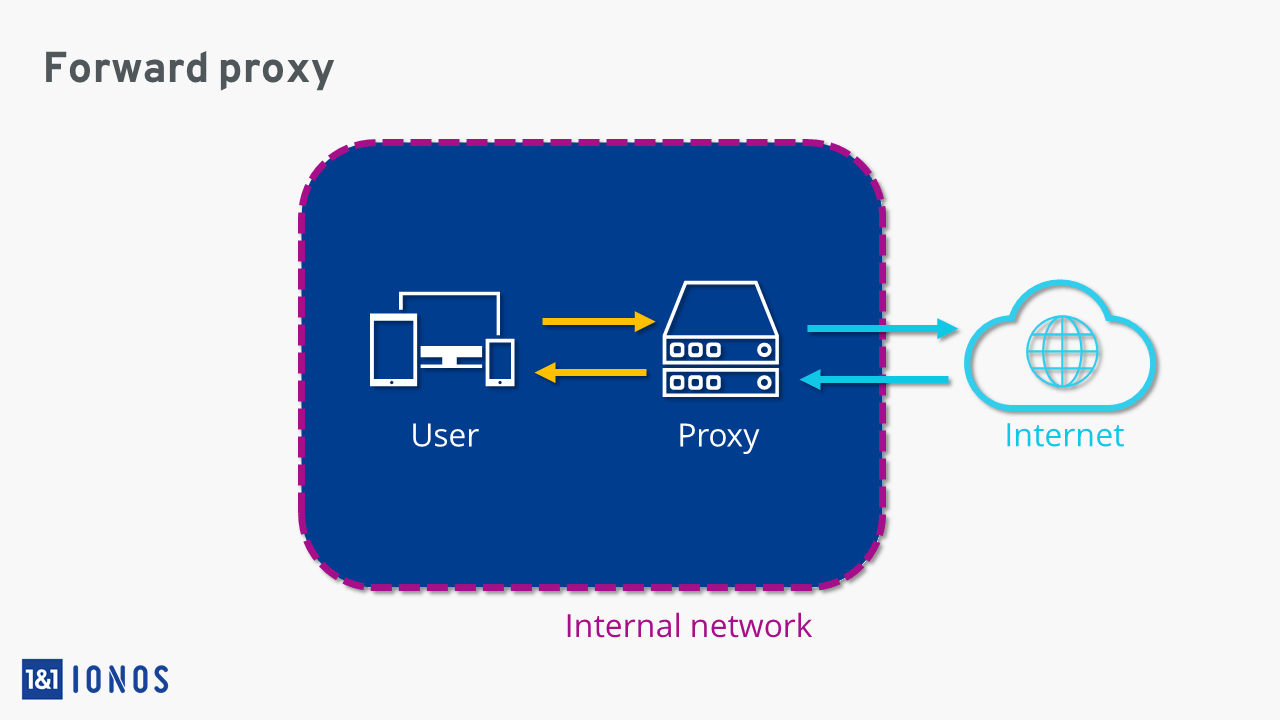
\includegraphics[width=0.45\textwidth]{imagenes/proxy}
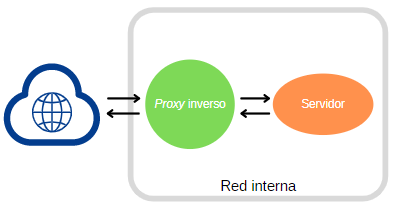
\includegraphics[width=0.45\textwidth]{imagenes/proxyInverso}
\caption{Esquema de un \emph{proxy} frente a un \emph{proxy} inverso. Imágenes de \url{https://www.ionos.es/digitalguide/servidores/know-how/que-es-un-servidor-proxy-inverso}.}
	\label{proxyContraProxyInverso}
\end{figure}

Como se puede inferir de las definiciones anteriores, el uso de un \emph{proxy} inverso no queda restringido a ciertas arquitecturas, pudiéndose utilizar para ocultar el servicio o servicios que consume cualquier aplicación. Sin embargo, este componente adquiere una gran importancia en el enfoque de microservicios, pues es importante no exponer estos al exterior. Además, se suele utilizar también para realizar tareas de balanceo de carga. La figura \ref{proxyInversoContraNoProxyInverso} muestra la comparativa de una arquitectura de microservicios básica y otra que utiliza el componente comentado. En la segunda se observa que con el uso de un \emph{proxy} inverso los clientes no acceden directamente a los microservicios, ni siquiera los conocen.

\begin{figure}[ht]
\centering
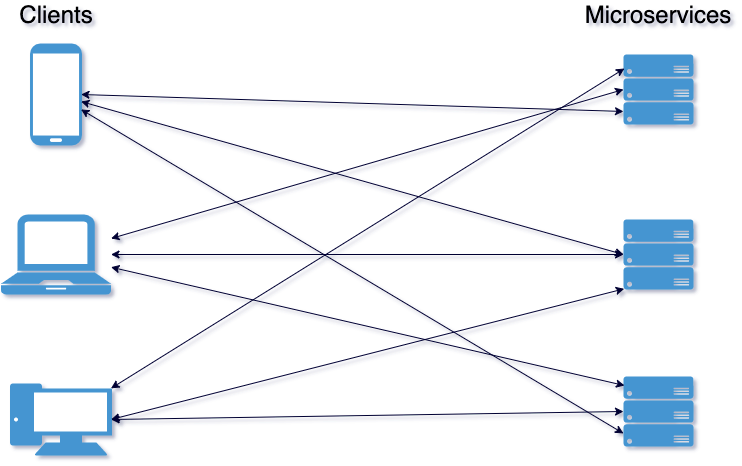
\includegraphics[width=0.45\textwidth]{imagenes/arquitecturaMicroserviciosBasica}
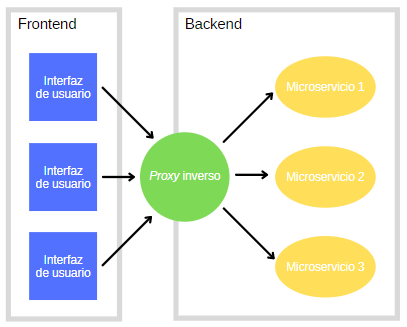
\includegraphics[width=0.45\textwidth]{imagenes/arquitecturaMicroserviciosConProxyInverso}
\caption{Arquitectura de microservicios básica frente a una con \emph{proxy} inverso. Imágenes de \url{https://www.adictosaltrabajo.com/2020/05/27/introduccion-al-api-gateway-pattern}.}
	\label{proxyInversoContraNoProxyInverso}
\end{figure}

	%%%%%%%%%%%%%%%%%%%%%%%%%%%%%% MOTIVACIÓN %%%%%%%%%%%%%%%%%%%%%%%%%%%%%%

	\section{Motivación}

La temática del trabajo es el desarrollo y despliegue de un \emph{proxy} inverso que actúe de intermediario entre la interfaz de usuario de la nueva aplicación en desarrollo y sus microservicios. Se pretende construir este nuevo componente porque se cree necesario proteger el \emph{backend} de la aplicación y ocultar los microservicios que lo forman. Por otro lado, también se quiere tener la posibilidad de lanzar a ejecución múltiples instancias de los microservicios con el fin de conseguir cierta tolerancia a fallos y poder también realizar balanceo de carga.

Este proyecto surge en el contexto de una práctica en empresa. El autor ha tenido la oportunidad de formar parte del equipo de I+D+i de una empresa de desarrollo de software enfocada al sector sociosanitario, durante un periodo de tiempo de más de un año. Esta empresa comercializa un software de gestión geriátrica y actualmente está desarrollando la nueva versión de su producto, utilizando enfoques y tecnologías de vanguardia, entre ellos: arquitecturas de microservicios, desarrollo de software dirigido por modelos y generación automática de código.

La temática comentada fue elegida debido a la estrecha relación que guarda con el desempeño del autor en las prácticas mencionadas, esto es, contribuciones a un microservicio específico destinado a orquestar el despliegue de la aplicación. Por otro lado, el desarrollo a llevar a cabo le va a otorgar una visión más global de la aplicación sobre la que se trabaja, así como aumentar el nivel de conocimiento acerca de la misma, con la motivación de seguir contribuyendo al proyecto por mucho tiempo más. Por último, la tecnología a utilizar, .NET, es de su interés y aspira así a crecer como desarrollador de ese \emph{framework}.

	%%%%%%%%%%%%%%%%%%%%%%%%%%%%%% OBJETIVOS %%%%%%%%%%%%%%%%%%%%%%%%%%%%%%

	\section{Objetivos}

El objetivo principal de este trabajo es construir un \emph{proxy} inverso. La construcción de este tiene las siguientes aspiraciones sobre la aplicación en construcción:

\begin{itemize}

\item \textbf{Ocultar los microservicios} que forman la aplicación para que la interfaz de usuario no acceda directamente a ellos por motivos de seguridad.

\item Permitir \textbf{múltiples instancias} en ejecución de los microservicios que, a su vez, tiene por finalidad:
\begin{itemize}

\item Conseguir que la aplicación sea \textbf{tolerante a fallos}, gracias a la posibilidad de tener un mismo microservicio desplegado en máquinas diferentes.

\item \textbf{Aumentar la eficiencia}, al poder crear o parar instancias dinámicamente según el tráfico que reciba la aplicación.

\end{itemize}

\end{itemize}

	%%%%%%%%%%%%%%%%%%%%%%%%%%%%%% ESTRUCTURA DEL DOCUMENTO %%%%%%%%%%%%%%%%%%%%%%%%%%%%%%

	\section{Estructura del documento}

?????

%%%%%%%%%%%%%%%%%%%%%%%%%%%%%% ESTADO DEL ARTE %%%%%%%%%%%%%%%%%%%%%%%%%%%%%%

\chapter{Estado del arte}

En la actualidad existen en el mercado muchas aplicaciones y servicios que se pueden utilizar como \emph{proxy} inverso. Algunas de estas soluciones son de pago, otras gratuitas e incluso algunas de código abierto. Se pueden dividir en dos tipos: productos \emph{software} ya construidos y librerías. Los primeros suelen ser fáciles de configurar y se pueden poner en marcha de una manera muy rápida. Las segundas requieren una parte de programación pero se adaptan mejor a las necesidades particulares, pues permiten tener más control al usuario. A continuación se van a comentar dos herramientas de cada tipo, una de las cuales será la tecnología utilizada. También se mostrará un ejemplo básico de uso de esta.

Cabe destacar que no hay muchos servicios que se dediquen exclusivamente a ofrecer un \emph{proxy} inverso. Estos suelen ofrecer otros productos como servidores web o balanceadores de carga. Por otro lado, lo habitual es hacer uso de un producto ya hecho, por lo que tampoco es fácil encontrar librerías que permitan personalizar un \emph{proxy} inverso, menos aún si hay que tener en cuenta la tecnología que se utiliza. En relación con esto, las librerías elegidas son para el lenguaje de programación C\#, utilizado en el resto de la aplicación de la que forma parte el \emph{proxy} inverso.

	%%%%%%%%%%%%%%%%%%%%%%%%%%%%%% API GATEWAY %%%%%%%%%%%%%%%%%%%%%%%%%%%%%%

	\section{API \emph{Gateway}}

A modo de aparte, es interesante mencionar un patrón parecido al \emph{proxy} inverso y que también podría haber sido utilizado para resolver el problema que atañe a este trabajo: el API \emph{Gateway}. Ambos comparten algunos casos de uso, por lo que sus diferencias causan confusión y no suelen quedar claras. Generalmente, se entiende que un API \emph{Gateway} es una especialización de un \emph{proxy} inverso, proporcionando así funcionalidades extra. Las más aceptadas e importantes son:

\begin{itemize}

\item Interpretan los mensajes que reciben y pueden hacer transformaciones sobre ellos; los \emph{proxy} inversos solo los redirigen donde corresponda.
\item Suelen ofrecer agregaciones de peticiones, esto es, aunar dos o más llamadas al \emph{backend} y exponer esta composición a través de un único \emph{endpoint}.
\item Realizan tareas transversales a todos los \emph{endpoints} como autenticación, autorización o monitorización.

\end{itemize}

El patrón recién comentado fue descartado desde el primer momento porque no se quería tener la funcionalidad de ninguno de los tres puntos clave que caracterizan esta aproximación. Por este motivo, y por la búsqueda de sencillez, era más coherente decantarse por un \emph{proxy} inverso.

	%%%%%%%%%%%%%%%%%%%%%%%%%%%%%% PRODUCTOS HECHOS %%%%%%%%%%%%%%%%%%%%%%%%%%%%%%

	\section{Productos hechos}

		%%%%%%%%%%%%%%%%%%%%%%%%%%%%%% NGINX %%%%%%%%%%%%%%%%%%%%%%%%%%%%%%

		\subsection{NGINX}

Originariamente NGINX \cite{NGINX} fue construido para ser un servidor web pero más tarde ofreció la posibilidad de actuar como \emph{proxy} inverso, balanceador de carga o \emph{proxy} para protocolos de correo electrónico. Desde la vertiente que interesa a este trabajo:

\begin{itemize}

\item Se trata de un \emph{proxy} inverso ligero y de alto rendimiento.
\item Ofrece una versión gratuita y otra de pago, NGINX Plus, la cual ofrece funcionalidades extra.
\item Se configura a través de un fichero el cual puede ser recargado durante su ejecución, es decir, se puede configurar dinámicamente.

\end{itemize}

		%%%%%%%%%%%%%%%%%%%%%%%%%%%%%% APACHE HTTPD %%%%%%%%%%%%%%%%%%%%%%%%%%%%%%

		\subsection{Apache HTTPD}

Apache HTTPD \cite{Apache}. Además de ser un servidor web "básico", y proveer contenido estático y dinámico a los usuarios finales, Apache HTTPD puede también actuar como proxy inverso

	%%%%%%%%%%%%%%%%%%%%%%%%%%%%%% LIBRERÍAS %%%%%%%%%%%%%%%%%%%%%%%%%%%%%%

	\section{Librerías}

		%%%%%%%%%%%%%%%%%%%%%%%%%%%%%% YARP %%%%%%%%%%%%%%%%%%%%%%%%%%%%%%

		\subsection{YARP}

YARP \cite{YARP} es una librería hecha por el propio Microsoft y su objetivo es facilitar la creación de \emph{proxies} inversos. Surgió dentro de la propia infraestructura de la empresa, en la que diferentes equipos preguntaban si existía algún \emph{proxy} inverso disponible para utilizar en sus respectivos proyectos. La respuesta de la compañía fue crear un equipo para construir esta librería y así estandarizar su uso. Además, se decidió hacer público tanto su uso como su código, siendo así una opción \emph{open source} a tener en cuenta.

Se encuentra todavía en desarrollo, habiendo sido lanzada su primera \emph{release} el 25 de Junio de 2020, y, a fecha de este trabajo, todavía solo se puede utilizar una \emph{preview}. Se prevé que vayan saliendo a la luz más versiones con más funcionalidades basadas en la experiencia de la propia empresa pero también en las opiniones de los usuarios externos. YARP es compatible con .NET Core 3.1 y .NET 5 pero algunas funcionalidades solo están disponibles para el segundo \emph{framework}, ya que se trata de la generación siguiente al primero.

A raíz de la heterogeneidad de casos de uso que debe cubrir para satisfacer las necesidades de los diferentes equipos de la compañía, está diseñada para ser muy personalizable y flexible. Otro aspecto importante es que permite cambiar la configuración del \emph{proxy} inverso de forma dinámica, lo que no obliga a tener que volver a lanzarlo a ejecución cuando se añada una nueva ruta, por ejemplo.

Permite construir \emph{proxies} inversos de nivel 7. Esto hace referencia a la capa del Modelo OSI (figura \ref{modeloOSI}) sobre la que actúan, la de aplicación en este caso. Gracias a esto, es posible modificar una petición HTTP antes de redirigirla, como por ejemplo sus \emph{headers} o ruta de destino. Sin embargo, no se puede hacer lo mismo con su contenido, ni siquiera es interpretado para tardar el menor tiempo posible en redirigir las peticiones. Además, no es un componente aparte sino que se integra con la \emph{pipeline} de \emph{middlewares} de .NET, haciendo que su eficiencia sea muy alta.

\begin{figure}[ht]
\centering
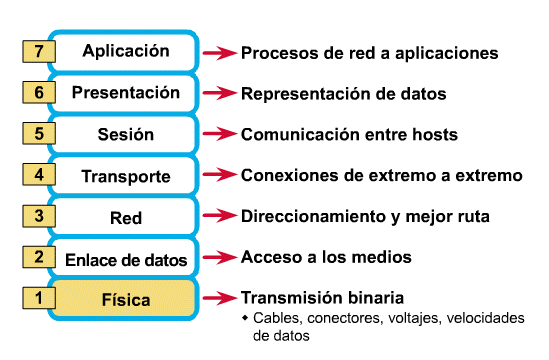
\includegraphics[width=0.8\textwidth]{imagenes/modeloOSI}
\caption{Modelo OSI.}
	\label{modeloOSI}
\end{figure}

Por último, la documentación propia no es corta pero tampoco excesiva. Asimismo, su corta edad hace que no se encuentren referencias o ejemplos de código de la comunidad fácilmente. Tampoco problemas planteados con sus posibles soluciones.

		%%%%%%%%%%%%%%%%%%%%%%%%%%%%%% OCELOT %%%%%%%%%%%%%%%%%%%%%%%%%%%%%%

		\subsection{Ocelot}
		
Ocelot \cite{Ocelot} es una librería para .NET Core que permite a una aplicación de ese \emph{framework} actuar como API \emph{Gateway}. Posee las características siguientes:

\begin{itemize}

\item Está pensada para arquitecturas orientadas a servicios o a microservicios.
\item Al tratarse de una librería, se utiliza de forma sencilla añadiéndola como un paquete NuGet más.
\item Su configuración es muy básica, teniendo que especificarla en un fichero Json.
\item No permite cambiar su configuración de manera dinámica.

\end{itemize}

	%%%%%%%%%%%%%%%%%%%%%%%%%%%%%% COMPARATIVA %%%%%%%%%%%%%%%%%%%%%%%%%%%%%%

	\section{Comparativa}

Precio, API Gateway, Reverse proxy, documentación, previa configuración, cantidad de configuración, extensibilidad, recarga de configuración dinámica.

	%%%%%%%%%%%%%%%%%%%%%%%%%%%%%% TECNOLOGÍA UTILIZADA %%%%%%%%%%%%%%%%%%%%%%%%%%%%%%

	\section{Tecnología utilizada}

Primero de todo, la tecnología utilizada es .NET, más concreto, el lenguaje de programación C\# y el entorno de desarrollo habitual para él, Visual Studio, en la versión del 2019. Como se comenta en la introducción de este capítulo, la aplicación en la cual se incluye el \emph{proxy} inverso está construida con ese \emph{framework}, por lo que se quiso mantener ese aspecto también en el nuevo componente.

Por otro lado, se ha decidido utilizar YARP para construir el \emph{proxy} inverso. La aplicación sobre la que se trabaja posee un mecanismo de despliegue automático muy 
particular, por lo que la flexibilidad y capacidad de adaptación que ofrece esta librería son muy adecuadas para integrar el \emph{proxy} inverso con dicho proceso. Si se hubiera utilizado un producto ya hecho, no se hubiera podido conseguir un nivel alto de cohesión y se hubieran tenido que abordar problemas de integración. Por otro lado, su sencillez y altas prestaciones hacen que destaque frente a Ocelot, la que, como ya se ha comentado, permite crear API \emph{Gateways}.

Por último, se ha utilizado Postman \cite{Postman} para realizar consultas de prueba al \emph{proxy} inverso y comprobar su funcionamiento. Postman es una herramienta gratuita que permite hacer justo lo que se ha descrito. Se trata de un cliente para peticiones HTTP REST que se utiliza para probar de manera sencilla servicios web y así agilizar su desarrollo.

		%%%%%%%%%%%%%%%%%%%%%%%%%%%%%% EJEMPLO DE USO BÁSICO %%%%%%%%%%%%%%%%%%%%%%%%%%%%%%

		\subsection{Ejemplo de uso básico}

Una vez comentado la elección que finalmente se hizo y el porqué, se va a introducir un ejemplo de uso básico de YARP para dar una visión general de lo que es capaz de hacer esta librería. De este modo, también será más fácil comprender el funcionamiento del \emph{proxy} inverso desarrollado.

En lineas generales, empezar a utilizar Yarp no es nada difícil, en un par de horas se puede llegar a tener un \emph{proxy} inverso básico funcionando, si bien es más complejo utilizar características avanzadas o personalizarlo en función de las necesidades particulares.

La demostración que se va a realizar consiste en crear un \emph{proxy} inverso que redirija peticiones hacía dos servicios web de prueba, creados anteriormente para el ejemplo. Estos simulan ser un servicio de localización y devuelven siempre \emph{Valencia, Spain}. También muestran este mismo mensaje por consola cuando son consultados.

Para empezar con el ejemplo, se crea un proyecto web vacío de .NET. Una vez el proyecto se ha creado, hay que añadir la referencia a la librería de YARP. En .NET las librerías se añaden como paquete NuGet y para buscar qué paquetes hay disponibles e instalarlos se puede utilizar un asistente gráfico, figura \ref{ejemploYARP_instalacionNuGet}.

\begin{figure}[ht]
\centering
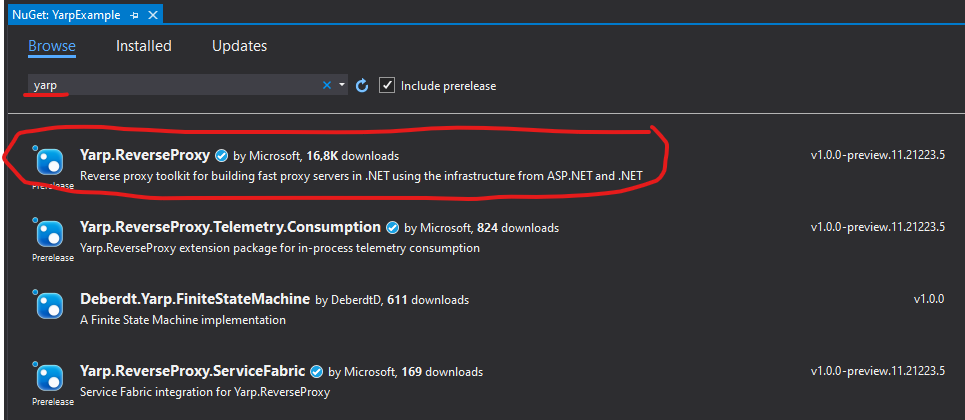
\includegraphics[width=1\textwidth]{imagenes/ejemploYARP/instalacionNuGet}
\caption{Instalación del NuGet de YARP.}
	\label{ejemploYARP_instalacionNuGet}
\end{figure}

Acto seguido, es necesario añadir un poco de código para poner en marcha un \emph{proxy} inverso sencillo. En la clase \emph{Startup} hay que modificar los métodos por defecto \emph{ConfigureServices} y \emph{Configure}. En el primero de ellos es necesario registrar el código del \emph{proxy} inverso, haciendo \emph{services.AddReverseProxy()}, y cargar la configuración de las rutas, \emph{proxyBuilder.LoadFromConfig()}. En el segundo basta con asegurarse de que se haga la llamada \emph{app.UseRouting()} y añadir  \emph{endpoints.MapReverseProxy()} dentro del \emph{UseEndpoint}. Para visualizar mejor estos cambios, figura \ref{ejemploYARP_startup}.

\begin{figure}[ht]
\centering
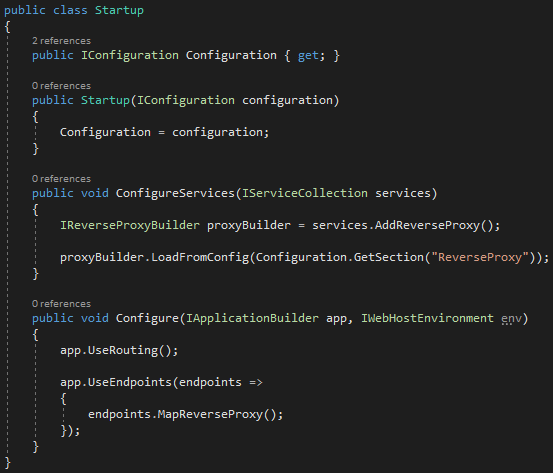
\includegraphics[width=0.7\textwidth]{imagenes/ejemploYARP/startup}
\caption{Clase \emph{Startup} después de añadir el código del \emph{proxy} inverso.}
	\label{ejemploYARP_startup}
\end{figure}

Por otro lado, hay que configurar las rutas que va a tener el \emph{proxy} inverso, es decir, los enrutamientos que debe hacer en tiempo de ejecución. Para ello se necesita especificar dichas rutas en el archivo \emph{appsettings}. Este archivo se utiliza para especificar cualquier tipo de configuración y se podría haber utilizado otro diferente. También se puede configurar a través de código pero requiere algo más de trabajo. Por este motivo, en esta demostración se va a utilizar el primer método, ya que se pretende mostrar un ejemplo lo más simple posible.

La figura \ref{ejemploYARP_appsettings} muestra las rutas creadas para esta demostración. Se ha creado un par ruta-\emph{cluster} con dos destinaciones. Para no entrar en mucho detalle, lo que es importante es que la ruta tiene un patrón \emph{\{**catch-all\}}, para capturar todas las peticiones, y el \emph{cluster} contiene dos destinaciones, una por cada servicio de localización, comentados al principio de este apartado. Lo que se pretende conseguir con esta configuración es que el \emph{proxy} inverso capture todas las peticiones y las envíe de manera aleatoria a cualquiera de los dos servicios de localización.

\begin{figure}[ht]
\centering
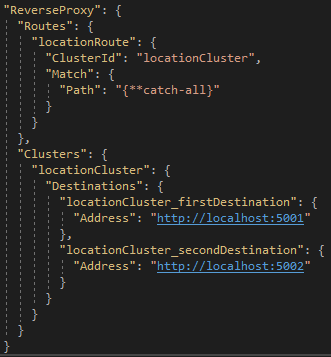
\includegraphics[width=0.50\textwidth]{imagenes/ejemploYARP/appsettings}
\caption{Fichero \emph{appsettings} con la configuración de las rutas.}
	\label{ejemploYARP_appsettings}
\end{figure}

Lo siguiente es preparar los servicios para una prueba rápida. En la figura \ref{ejemploYARP_servicios_preparacion} se observa el escenario inicial. En la parte superior se encuentra el \emph{proxy} inverso creado y, en la inferior, los dos servicios de localización . Importante destacar que los puertos de estos últimos coinciden con lo que se han indicado en el \emph{appsettings}.

\begin{figure}[ht]
\centering
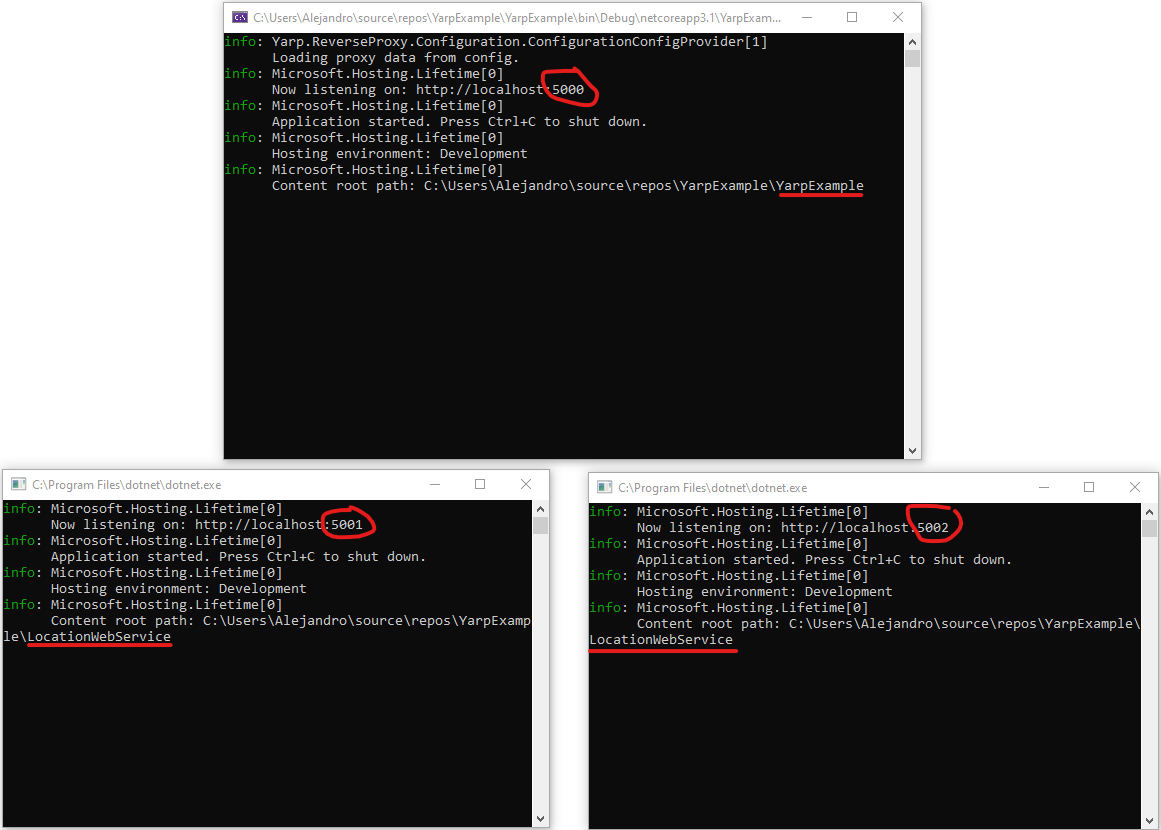
\includegraphics[width=1\textwidth]{imagenes/ejemploYARP/servicios_preparacion}
\caption{Escenario inicial con los servicios preparados.}
	\label{ejemploYARP_servicios_preparacion}
\end{figure}

Para simular una petición de un cliente se va a realizar una consulta con Postman. Esta estará dirigida al \emph{proxy} inverso y deberá ser redirigida a alguno de los dos servicios de localización, como se ha indicado en el \emph{appsettings}. En la figura \ref{ejemploYARP_servicios_funcionando}, se muestra el escenario anterior tras ejecutar la petición Postman repetidas veces. Se observa que el \emph{proxy} inverso la ha redirigido de manera aleatoria entre los dos otros servicios. En la consola del \emph{proxy} inverso es interesante ver el mensaje por defecto que muestra YARP indicando hacia qué dirección redirige cada petición.

\begin{figure}[ht]
\centering
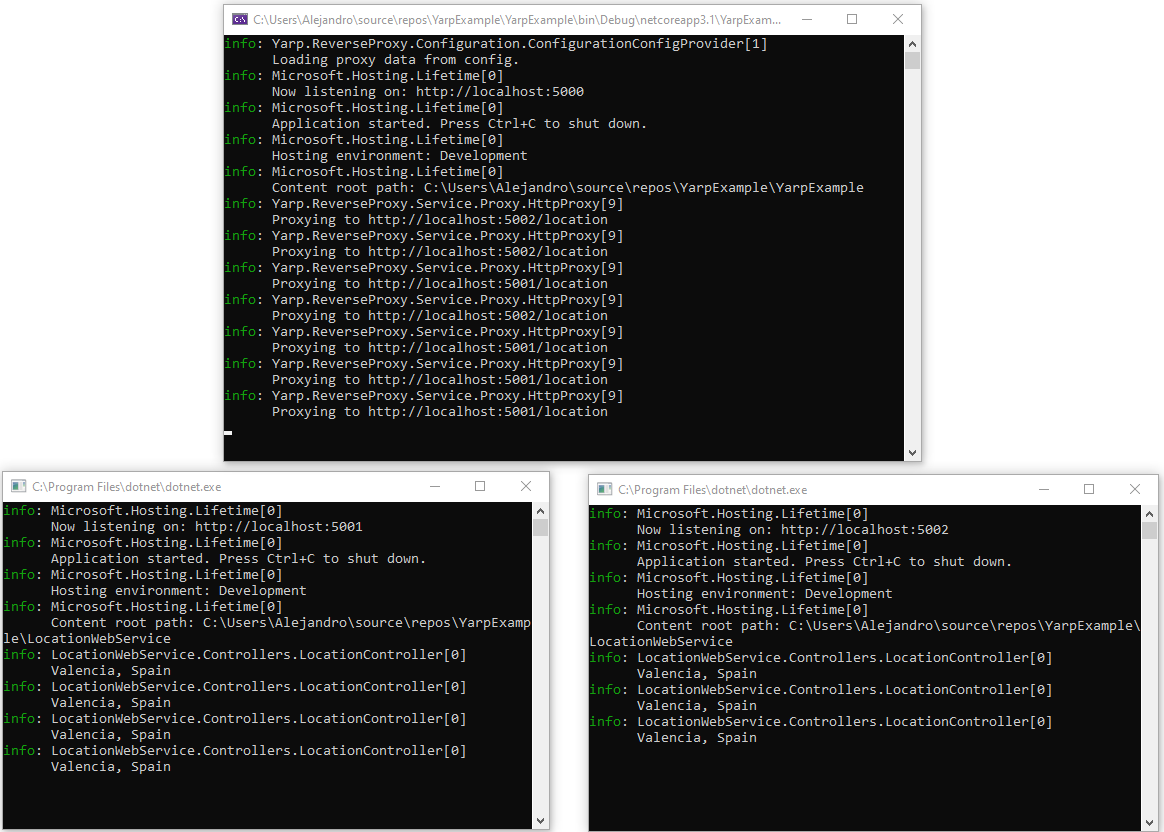
\includegraphics[width=1\textwidth]{imagenes/ejemploYARP/servicios_funcionando}
\caption{Escenario con los servicios después de realizar algunas consultas.}
	\label{ejemploYARP_servicios_funcionando}
\end{figure}

%%%%%%%%%%%%%%%%%%%%%%%%%%%%%% DESARROLLO DE LA SOLUCIÓN %%%%%%%%%%%%%%%%%%%%%%%%%%%%%%

\chapter{Desarrollo de la solución}

?????

	%%%%%%%%%%%%%%%%%%%%%%%%%%%%%% ESPECIFICACIÓN DE REQUISITOS %%%%%%%%%%%%%%%%%%%%%%%%%%%%%%

	\section{Especificación de requisitos}

\begin{itemize}

\item Redirección de peticiones
\item Carga dinámica de rutas
\item Eliminación de rutas
\item Instancia múltiple de microservicios
\item Versionado de microservicios

\end{itemize}

		%%%%%%%%%%%%%%%%%%%%%%%%%%%%%% CASOS DE USO %%%%%%%%%%%%%%%%%%%%%%%%%%%%%%

		\subsection{Casos de uso}

?????

		%%%%%%%%%%%%%%%%%%%%%%%%%%%%%% PRUEBAS DE ACEPTACIÓN %%%%%%%%%%%%%%%%%%%%%%%%%%%%%%

		\subsection{Pruebas de aceptación}

?????

	%%%%%%%%%%%%%%%%%%%%%%%%%%%%%% DISEÑO %%%%%%%%%%%%%%%%%%%%%%%%%%%%%%

	\section{Diseño}

?????

		%%%%%%%%%%%%%%%%%%%%%%%%%%%%%% DIAGRAMA DE COMPONENTES %%%%%%%%%%%%%%%%%%%%%%%%%%%%%%

		\subsection{Diagrama de componentes}

?????

		%%%%%%%%%%%%%%%%%%%%%%%%%%%%%% DIAGRAMA DE CLASES %%%%%%%%%%%%%%%%%%%%%%%%%%%%%%

		\subsection{Diagrama de clases}

?????

	%%%%%%%%%%%%%%%%%%%%%%%%%%%%%% METODOLOGÍA %%%%%%%%%%%%%%%%%%%%%%%%%%%%%%

	\section{Metodología}

?????

	%%%%%%%%%%%%%%%%%%%%%%%%%%%%%% PROGRAMACIÓN %%%%%%%%%%%%%%%%%%%%%%%%%%%%%%

	\section{Programación}

La construcción del \emph{proxy} inverso que protagoniza este trabajo ha pasado por una serie de etapas que se van a comentar a continuación.

		%%%%%%%%%%%%%%%%%%%%%%%%%%%%%% CONSTRUCCIÓN DE PROTOTIPOS %%%%%%%%%%%%%%%%%%%%%%%%%%%%%%

		\subsection{Construcción de prototipos}

El desarrollo comenzó con la elaboración de dos prototipos de microservicio con la funcionalidad mínima para redirigir peticiones. Estos prototipos tenían la misión de demostrar si era posible seguir la estructura general de todos los microservicios de la aplicación, con gran parte del código generado a partir de modelos. Precisamente este código autogenerado es lo que generaba ciertas dudas con lo referente al rendimiento final, el cual se podía ver perjudicado debido a un código menos específico y más genérico, así como a un exceso de características innecesarias para el caso en cuestión pero que sí debían poseer el resto de microservicios.

El primero de los prototipos se hizo lo más simple posible, es decir, con la lógica justa y necesaria para desempeñar su trabajo y sin seguir ninguna estructura concreta. El segundo, fue construido utilizando las mismas herramientas con las que fueron construidos el resto de microservicios de la aplicación, esto es, generación de código a partir de modelos. Cabe destacar que, para no realizar esfuerzos en vano sin saber qué prototipo iba a ser la opción elegida, se dejaron algunos detalles correspondientes a la generación de código pendientes. Esto se debe a que el proceso de generación de código no se adaptaba al cien por cien a las necesidades del nuevo microservicio.

Una vez construidos los prototipos, se procedió a medir el impacto de seguir la norma para decidir qué prototipo desechar y con cuál seguir adelante.

Los resultados de las mediciones fueron claros: ambos prototipos tenían un rendimiento casi idéntico. De esta forma, se decidió continuar con la versión autogenerada.

		%%%%%%%%%%%%%%%%%%%%%%%%%%%%%% CONSOLIDACIÓN DEL MICROSERVICIO AUTOGENERADO %%%%%%%%%%%%%%%%%%%%%%%%%%%%%%

		\subsection{Consolidación del microservicio autogenerado}

Una vez elegida la opción de seguir el estándar, hubo que resolver los aspectos de la generación de código que no quedaron resueltos. Así pues, se tuvo que modificar algunas plantillas de código a partir de las cuales se generan los microservicios. Por otro lado, también fue necesario abordar otros problemas derivados de seguir el patrón de microservicio estándar.

		%%%%%%%%%%%%%%%%%%%%%%%%%%%%%% PRIMEROS DESPLIEGUES %%%%%%%%%%%%%%%%%%%%%%%%%%%%%%

		\subsection{Primeros despliegues}

A estas alturas del desarrollo ya se tenía una primera versión del \emph{proxy} inverso perfectamente funcional pero antes de llevar a cabo los primeros despliegues había que adaptarlo al proceso de despliegue que se seguía hasta el momento. La interfaz de usuario de la aplicación se conectaba directamente a los microservicios por lo que hizo falta interponer el nuevo componente entre ella y el \emph{backend}.

Más tarde, se hizo que los propios microservicios utilizaran el \emph{proxy} inverso para comunicarse entre ellos.

El único microservicio que no se pudo reemplazar fue el de autorización porque tenía una dirección específica, configurada a través del DNS.

Como paso previo a incluir el \emph{proxy} inverso al proceso de despliegue primero se hicieron pruebas de manera local. Se desplegó el \emph{proxy} inverso en una máquina a parte y se le cargó con rutas que apuntaban a los microservicios ya desplegados para que la interfaz de usuario lo utilizara. Se comprobó que todo funcionaba correctamente.

Un problema que surgió fue el de los timeouts. Dos microservicios tenían un timeout muy grande debido al elevado coste de sus peticiones. El \emph{proxy} inverso cortaba las llamadas antes de que terminaran. Al final esto resultó culpa de \emph{YARP}, que tiene un timeout por defecto de 100 segundos. La solución fue aumentar el timeout para las peticiones que se dirigen a los microservicios en cuestión. Para ello, fue necesario añadir un parámetro opcional para el timeout en la creación de rutas. De esta forma se permite la personalización del timeout en función de la ruta que se utilice.

	%%%%%%%%%%%%%%%%%%%%%%%%%%%%%% PRUEBAS %%%%%%%%%%%%%%%%%%%%%%%%%%%%%%

	\section{Pruebas}

Para comprobar el correcto funcionamiento del \emph{proxy} inverso se han realizado dos tipos de pruebas: unas más sencillas, hechas cada vez que se producía un incremento considerable de funcionalidad, y otras más formales, al final del proyecto.

		%%%%%%%%%%%%%%%%%%%%%%%%%%%%%% PRUEBAS DE REGRESIÓN %%%%%%%%%%%%%%%%%%%%%%%%%%%%%%

		\subsection{Pruebas de regresión}

Se trata de una serie de comprobaciones definidas formalmente que han servido para verificar que las funcionalidades anteriormente implementadas no dejaban de funcionar al añadir nuevas.

		%%%%%%%%%%%%%%%%%%%%%%%%%%%%%% PRUEBAS FINALES %%%%%%%%%%%%%%%%%%%%%%%%%%%%%%

		\subsection{Pruebas finales}

Con el propósito de garantizar la corrección del comportamiento del producto \emph{software} desarrollado se llevaron a cabo pruebas finales. A las pruebas de regresión anteriormente comentadas se les añade...

%%%%%%%%%%%%%%%%%%%%%%%%%%%%%% CONCLUSIONES %%%%%%%%%%%%%%%%%%%%%%%%%%%%%%

\chapter{Conclusiones}

Decir si los objetivos se han cumplido.

En un futuro se puede querer extender la funcionalidad y convertirlo en un API \emph{Gateway}.

%%%%%%%%%%%%%%%%%%%%%%%%%%%%%% BIBLIOGRAFÍA %%%%%%%%%%%%%%%%%%%%%%%%%%%%%%

\begin{thebibliography}{10}

\bibitem{LewisAndFowler}
Artículo de J. Lewis y M. Fowler acerca de los microservicios.
\newblock Disponible en:\\
\url{https://martinfowler.com/articles/microservices.html}

\bibitem{Newman}
Libro de referencia sobre microservicios:\\
\newblock Sam Newman,
\newblock \emph{Building Microservices}

\bibitem{NGINX}
¿Cómo utilizar NGINX como proxy inverso?:\\
\url{https://docs.nginx.com/nginx/admin-guide/web-server/reverse-proxy}

\bibitem{Apache}
¿Cómo utilizar Apache HTTPD como proxy inverso?:\\
\url{https://httpd.apache.org/docs/trunk/es/howto/reverse_proxy.html}

\bibitem{YARP}
Sitio oficial de YARP:\\
\url{https://microsoft.github.io/reverse-proxy}

\bibitem{Ocelot}
Sitio oficial de Ocelot:\\
\url{https://threemammals.com/ocelot}

\bibitem{Postman}
Sitio oficial de Postman:\\
\url{https://www.postman.com}

\end{thebibliography}

\end{document}
